\section{Evaluation}
\label{sec:eval}

To evaluate Shadowfax, we focused on six key questions:
\begin{enumerate}
\item {\bf Does it preserve \faster{}'s performance?}
  \S\ref{sec:eval:clients} shows that Shadowfax preserves \faster{}'s
  scalability and adds in negligible overhead.
%
  Its throughput scales to 130~Mops/s on 64~threads on a VM even when using
  Linux TCP.

\item {\bf How does it compare to an alternate design?}
  \S\ref{sec:eval:clients} shows that Shadowfax performs 4x better than
  a state-of-the-art approach that partitions dispatch as well as data.

\item {\bf Does it provide low latency?}
  \S\ref{sec:eval:latency} shows that while serving a throughput of 130~Mops/s,
  Shadowfax's median latency is 1.3~ms on Linux TCP.
%
  Using two-sided RDMA decreases this to 40~\us.

\item {\bf Can it maintain high throughput during scale out?}
  In \S\ref{sec:eval:migration}, we see that when migrating 10\% of a server's
  hash range, Shadowfax's scale-out protocol can maintain throughput
  above 80~Mops/s.
%
  Parallel data migration can help complete scale out in under 17~s,
  and sampled records help recover throughput 30\% faster
  (\S\ref{sec:eval:sampling}).

% \item[Can sharding be lazy and flexible?]
%   \S\ref{sec:eval:migration:views} shows that view validation has lower
%   runtime overhead compared to hash validation, which can deteriorate
%   throughput by upto 17\%.
%
%   When coupled with fast migration, this allows Shadowfax to be lazy and
%   flexible about how it distributes load.

\item {\bf Do indirection records help scale out?}
  \S\ref{sec:eval:migration:indir} shows
  that by restricting migration to main memory, indirection records help
  speed scale out by 6x.
%
  They also have a negligible impact on server throughput once scale out
  completes.
% , but at the cost of larger migrations.
%
% They have a negligible impact on normal case throughput, but result
% in larger pending queues.
%
% They can be cleaned up during compaction with no additional overhead.

\item {\bf Do views reduce scale out's impact on normal operation?}
  In \S\ref{sec:eval:migration:views}, we show that validating ownership
  using views has a negligible impact on normal case server throughput.
%
  When compared to hash validating each request within a batch, views
  improve throughput by as much as 17\% depending on the number of hash
  ranges owned by the server.

\item {\bf Can it scale across scales?}
  \S\ref{sec:eval:system-scalability} shows that when scaled across
  machines, Shadowfax continues to retain \faster's high throughput.
%
  A cluster consisting of 768 threads spread across 12 servers scales
  linearly to 930~Mops/s while servicing 2304 client sessions.

\end{enumerate}

% We also ran Shadowfax on a small
% CloudLab~\cite{cloudlab} cluster consisting of 256 cores spread across 8
% servers
% and found that its throughput scales linearly to 400~Mops/s.
%
% We omit this experiment from this paper because of a lack of space.

\subsection{Experimental Setup}

We evaluated Shadowfax on the Azure public cloud~\cite{azure}.
%
We ran all experiments on the E64\_v3 series of virtual
machines~\cite{e64} (Table~\ref{table:exptconfig}).
%
Experiments use 64 cores unless otherwise noted.
%
Each VM uses accelerated networking, which offloads
much of the networking stack onto FPGAs~\cite{accel-nw}, allowing us to
evaluate Shadowfax over regular Linux TCP.
%
Shadowfax's remote tier uses Azure's paged blobs on premium
storage~\cite{page-blobs}, which offer 7,500 random IOPS with a write
throughput of 250~MB/s per blob.

We used a dataset of 250~million records, each consisting of
an 8~byte key and 256~byte value (totalling 80~GB in Shadowfax).
%
To evaluate the system under heavy ingest, we used YCSB's F
workload~\cite{ycsb} consisting of read-modify-write requests.
%
Each request reads a record, increments a counter within the record, and
writes back the result.
%
This counter could represent heartbeats for a sensor device, click
counts for an advertisement or views/likes on a social media profile.
%
Unless noted, requested keys follow YCSB's default Zipfian distribution ($\theta = 0.99$).

We compare to two baselines; one representing the
state-of-the-art in fast request processing, the other representing the
state-of-the-art in data migration.

\begin{enumerate}
\item \textbf{Seastar+Memcached}~\cite{seastar}
is an open-source framework for building high
performance multi-core services.
%
Its shared-nothing design constrasts with Shadowfax;
servers partition data across cores, eliminating the need for locking.
%
Clients can send requests to any server thread;
Seastar uses message passing via shared memory queues to route
each request to the core that processes requests for that data item.
%
Seastar represents a best case for the state-of-practice; it is highly optimized.
%
It uses lightweight, asynchronous futures to avoid
context switch overheads, and it uses advanced NIC features like
FlowDirector~\cite{flow-director} to partition and scale network processing.
%
We used an open-source, lock-free, shared-nothing version of
Memcache on Seastar as a baseline~\cite{seastar-apps}.
%
We batched 100 operations per request, which maximized its throughput.

\item \textbf{Rocksteady}~\cite{rocksteady} is a state-of-the-art migration
protocol for RAMCloud~\cite{ramcloud}.
%
To accelerate migration, it immediately routes requests for migrated records
to the target, while it is transfering records (which only reside in memory).
%
It slowly performs disk I/O in the background to incorporate the migrated records
into durable, on-disk replicas that belong to the target; this must complete
before the source and target can be independently recovered.
%
%A temporary, coarse-grained dependency between the source and
%target's on-disk data ensures fault tolerance if either machine
%crashes.
%
We modified Shadowfax to use a similar approach as a baseline.
%
Instead of using indirection records, first, all in-memory records are moved;
then, the source performs a sequential scan over all records on durable
storage, where all encountered live are sent to the target.
%
%Like in Rocksteady, the source and target stay coupled together for
%fault-tolerance during this phase.
%
%Once it completes, migration is completed, and they can be decoupled
%using Shadowfax's 2PC based mechanism.
\end{enumerate}

\subsection{Throughput Scalability}
\label{sec:eval:clients}

Shadowfax partitions request dispatching across threads for
performance.
%
It shares access to \faster between threads to provide high
throughput even under skew.
%
To demonstrate this, we measured throughput while scaling the number of threads
on one server machine with one client machine.
%
The entire dataset resides in memory, ensuring the experiment is CPU-limited.
%
Figure~\ref{fig:thread-scalability} shows the results on Shadowfax, on
\faster when requests are generated on the same machine (i.e., no networking involved), and on Shadowfax without
hardware accelerated networking.

%{\color{red} RS: I think we need to be a bit careful here; is there a way we
%can word this paragraph still to reinforce that we aren't partitioning data or network
%load in any particular way?}
%
Shadowfax retains \faster{}'s scalability.
%
\faster{} scales to service 128~Mops/s on 64 threads.
%
Adding in the dispatch layer and remote client preserves performance;
Shadowfax scales to 130~Mops/s on 64 threads.
%
This is because it avoids cross thread synchronization or communication for
request processing from the point a client thread issues a request until the
server thread executes it on \faster.
%
Client threads' pipelined batches of asynchronous requests also avoid any
slowdown from stalls induced by network delay, keeping all threads at the
client and server busy at all times.

Hardware network acceleration also plays an important role in
maintaining performance; when disabled, throughput reaches only 58\%
(75~Mops/s) of
accelerated TCP.
%
Here, CPU overhead for TCP transport processing increases, so the server
slows due to additional time spent in \texttt{recv()} syscalls instead of doing
work.
%
Hardware acceleration offloads a significant portion of packet processing to a
SmartNIC, allowing Shadowfax to maintain \faster{}'s scalability without
relying on kernel-bypass networking (DPDK or RDMA).

Next, we compared Shadowfax to Seastar
(Figure~\ref{fig:thread-scalability-comparison}) using a uniform key access
distribution; this is the only distribution that Seastar's client harness
supports (this advantages Seastar's shared-nothing approach, which suffers
imbalance under skew).
%
Seastar scales to 10~Mops/s on 28 threads, after which throughput is flat.
%
Shadowfax scales linearly to 85~Mops/s on 64 threads; even at 28 threads, it is
already 4x faster than Seastar.
%
This is because Seastar partitions work at the wrong layer; threads maintain
independent indices to avoid synchronizing on records, but this forces threads
to use inter-core message passing when they receive a request to route it to
the thread that has that record.
%
To ensure that this is the case and that it is not the result of a bottleneck in
Seastar's shared-nothing memcached implementation, we also measured the
throughput of Seastar's when each request is a no-op (by disabling its index,
see Seastar-NOP).
%
This improves Seastar's throughput, but it is still 4$\times{}$ slower
than Shadowfax on 64 threads.
%
This reinforces that simply attaching more scalable index like
\faster to Seastar's networking and dispatch layers is not sufficient to get
good performance; forced cross-core routing of requests is the bottleneck.

In contrast, Shadowfax's design helps it exploit its shared \faster instance,
which is lock-free and minimizes cache footprint.
%
It leaves all synchronization and communication to the hardware
cache coherence, which is more efficient than explicit software
coordination and only incurs high costs when real contention arises in data
access patterns, rather than pessimistically synchronizing on all requests.
%
Shadowfax's advantage grows with skew;
Figure~\ref{fig:thread-scalability} shows its performance improves by 1.5x
under skew, whereas Seastar's performance would decrease.
%
%Seastar's client harness does not support generating a Zipfian
%distributed workload, but partitioning data records leads to load
%imbalance across threads under high skew, and hurts throughput.
%
%Because it avoids such imbalances and uses a highly optimized index,
%Shadowfax's throughput improves by 1.5x on moving from a uniform to a
%Zipfian distribution.

In addition to Azure TCP, we also measured Shadowfax's scalability on
Azure Infrc and on CloudLab~\cite{cloudlab}.
%
Figure~\ref{fig:acceleration} demonstrates that Shadowfax's throughput
scales linearly on these platforms too.

\subsubsection{Insert only workload}
\label{sec:eval:append-only}

\faster's \hlog is key to Shadowfax's high throughput since it allows
records to be updated in-place.
%
However, in-place updates might not always be possible.
%
For workloads that are insert only, throughput will be limited by the
rate at which records can be appended to the \hlog's tail.
%
Figure~\ref{fig:thread-scalability-append} presents scalability for
such a workload.
%
Throughput scales to 8~Mops/s on 16 threads.
%
Beyond 16 threads, increments to the \hlog's tail bottleneck the system,
and throughput saturates.

\subsection{Batching and Latency}
\label{sec:eval:latency}

Shadowfax clients send requests in pipelined batches to amortize
network overheads and keep servers busy.
%
Asynchronous requests with hardware network acceleration
help reduce batch sizes and latency.
%
To show this, we measured its median latency and batch size at
server saturation.
%
%
Table~\ref{table:latency} presents results on TCP, TCP with
hardware acceleration disabled, and with two-sided RDMA (Infrc).
%
We used Azure's HC44rs~\cite{hc44} instances for Infrc, since they support
(100~Gbps) RDMA; they have Xeon Platinum 8168 processors with 44 vCPUs.
%
% These instances are able to saturate Shadowfax at 44 vCPUs
% itself.
%
% This is because Shadowfax is compute bound under our workload, and
% cores on the Infrc instances can simultaneously turbo boost to 3.7~GHz
% compared to 2.6~GHz on the TCP instances.
%
% As a result, they can saturate throughput with fewer vCPUs.

Most of Shadowfax's latency comes from batching, which amortizes network CPU
costs. Accelerated networking reduces CPU load, decreasing the batching
needed to retain throughput.
%
%The asynchronous client library prevents threads from blocking while
%waiting for these in-flight batches to complete at the server, and
%allows them to continue issuing requests into session buffers.
%
Accelerated networking keeps the batch size required to saturate
throughput small at 32~KB, which also keeps median latency low at 1.3~ms.
%
%With hardware acceleration disabled, the software network stack now
%becomes a bottleneck (\texttt{recv()}).
%
Without acceleration, increased batch size doesn't help; with 32~KB
batches throughput drops to 75~Mops/s, and median latency increases to 2.2~ms.

Predictably, the batch size required to saturate throughput on Infrc is
significantly lower at 1~KB, dropping median latency to 40~\us.
%
This is because the network is faster and the stack is implemented in hardware;
servers and clients can receive and transmit batches with near-zero
software overhead (including system calls).
%
Secondly, vCPUs on these instances are faster; they have a base clock rate of
2.7~GHz compared to 2.3~GHz on the TCP instances
(Table~\ref{table:exptconfig}).
%
This speeds servers and clients, reducing the batch size and
threads (from 64 to 44) required to reach the same throughput.

To evaluate this further, we ran Shadowfax using TCP over IPoIB~\cite{ipoib} on
the Infrc instances (Table~\ref{table:latency}, TCP-IPoIB).
%
Throughput still saturates at 125~Mops/s.
%
Compared to hardware accelerated TCP, faster vCPUs reduce the batch size
by 4x (8~KB) and median latency by 5x (260~\us).
%
Differences in the network might also contribute to these improvements,
but we found Shadowfax to be CPU-bound in both cases.

%This demonstrates an important benefit of Shadowfax's design.
%
%Instead of improving performance by increasing
%client fan-in at a server, the system can be sped up by
%simply improving performance at each thread; either by using faster
%vCPUs (cores) or by optimizing software.

% \subsection{Transparent Multi-Tiered Storage}
% \label{sec:eval:dfs}
% \begin{figure}[t]
% \centering
% 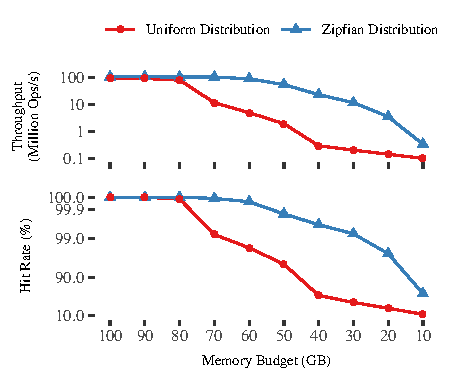
\includegraphics[width=\columnwidth]{
%     sofaster-data/memory-budget/memory-budget.pdf}
% \caption{Shadowfax throughput under decreasing memory budgets. Under a
%     Zipfian access pattern, it can sustain high throughput under
%     small budgets because of a small working set that fits in memory.}
% \label{}
% \end{figure}
%
% \begin{figure}[t]
% \centering
% \includegraphics[width=\columnwidth]{
%     sofaster-data/memory-budget/memory-budget-disk.pdf}
% \caption{}
% \label{}
% \end{figure}

\subsection{Memory Budget}
\label{sec:eval:dfs}

% \begin{figure}[t]
% \centering
% \includegraphics[width=\columnwidth]{
%     sofaster-data/memory-budget/memory-budget-disk.pdf}
% \caption{}
% \label{}
% \end{figure}

\faster's throughput eventually becomes limited by the SSD when the
entire dataset does not fit in main memory.
%
Shadowfax's dispatch layer and client library ensure
that this does not change when requests are generated over the cloud
network.
%
To show this, we measured throughput under a decreasing main-memory
budget for the \hlog.
%
We also measured the hit rate (the percentage of requests
that were served from main-memory) during this experiment.
%
Figure~\ref{fig:memory} presents the results
(in log scale).

Overall, throughput drops as the memory budget decreases.
%
This is because the system needs to issue random IO to fetch records
from SSD.
%
Once fetched, these records are appended to the \hlog's tail which
flushes records at its head to SSD leading to more random IO during
future requests.
%
For a uniform distribution, throughput begins to drop at
80~GB.
%
Since all records are equally hot, even a small set on SSD hurts the hit
rate and saturates SSD IOPS (Table~\ref{table:exptconfig}).
%
For a zipfian distribution, a smaller hot set ensures that this
begins to happen only at 50~GB.
%
Throughput still drops because of low SSD IOPS
(Azure throttled our VMs to 96,000 IOPS), decreasing to 3.5~Mops/s at 20~GB.
%
However, this is still 24$\times{}$ better than the uniform case which
drops to 0.146~Mops/s.

\subsection{Scale Out}
\label{sec:eval:migration}

Shadowfax's migration transfers hash ranges between
two machines and minimizes throughput impact while doing so.
%
Indirection records help restrict migration to memory, speeding up
scale out, decoupling the source and target sooner.
%
To demonstrate this, we measured throughput during scale up.

In a 5-minute experiment with one client and two servers (a source and a
target), the entire hash space initially resides at the source.
%
After one minute, 10\% of this hash range is moved to the target.
%
Figure~\ref{fig:migration} shows system throughput during
the experiment; Figure~\ref{fig:migration-split}
shows source and target throughput separately.
%
In (a), all records are placed in memory.
%
In (b) and (c), servers are restricted to a memory budget of 60~GB,
allowing us to compare the impact of indirection records (in (b)) against
Rocksteady's scan-the-log approach (in (c)).

\subsubsection{All-In-Memory Scale Out}

Global cuts for ownership transfer avoid stalling cores at migration start, but
the view change for this cut has some impact; request batches are invalidated,
causing requests to be shuffled among sessions buffers at the client
(we calculated the number of such requests to be approximately 250,000).
%
This is visible in Figure~\ref{fig:migration} (a); throughput at the
start of scale out (1 minute) briefly drops to 80~Mops/s.

Figure~\ref{fig:migration-split} (a) shows that throughput on the source
stays at 85~Mops/s after this.
%
This is because the source is collecting and transmitting records as it
services requests.
%
Parallel migration limits the length of this impact in two ways.
%
First, it accelerates migration, completing in 17~s and restoring full
throughput.
%
Second, as more records shift to the target, it
serves more requests, causing system throughput to recover
even before scale up completes.
%
Once scale up completes, system throughput increases by 10\% as expected.

Shadowfax's asynchronous client library helps limit the
impact too.
%
When the target receives a request for a record that has not been
migrated yet, it marks the request as pending.
%
This keeps clients from blocking, allowing them to
continue sending requests.
%
To prevent a buildup of pending requests, the target periodically tries to complete them.
%
Figure~\ref{fig:comparison-pending} (a) shows the number of pending operations at the
target during migration.
%
When migration starts, requests flood the target, pending 100 million requests.
%
As records migrate, these requests complete, with the last pending operation
completing 100~s after migration start.
%
Hence, practical migrations must be small and incremental to bound
delay; however, throughput recovery is more important in Shadowfax's target
applications whereas latency can be tolerated with asynchrony.

We also ran the above experiment on a larger cluster of four 64 core machines
on CloudLab~\cite{cloudlab} and obtained similar results; aggregate cluster
throughput in that experiment was only impacted by 20\% in the worst case
during migration, since throughput is only reduced at the source during
migration.

\subsubsection{Indirection Records}
\label{sec:eval:migration:indir}

With a 60~GB memory budget, some records to be migrated are on the source's
SSD.
%
Rocksteady's approach (Figure~\ref{fig:migration} (c)) migrates records from
memory and then scans the on-SSD log to migrate colder records.
%
Parallel migration completes the in-memory phase in just 14~s.
%
Thoughput improves quickly after this phase, since these are hotter records.
%
However, the second phase is single threaded, scans over files on SSD,
and takes 165~s to complete.
%
Hence, scale out takes 180~s, and the source and target remain inter-dependent
for fault tolerance.

Indirection records solve this, completing migration in 32~s
(Figure~\ref{fig:migration} (b)) and decoupling the source and target 6x faster.
%
By sending out records that point to shared remote storage, migration
is restricted to memory and avoids I/O at the source altogether.
%
%
However, this approach increases the amount of data transmitted to the target.
%
Figure~\ref{fig:migration-size} show this effect.
%
Compared to Rocksteady's 5.60~GB, indirection records cause
16.47~GB to be transmitted from memory to the target.
%
This is because we must send about one indirection record per hash table bucket
entry, totaling 11~GB here.
%
%We leave improving this algorithm to future work.
%
The larger migration takes 18~s longer than Rocksteady's in-memory phase, but it
decreases the total duration of migration by 150~s.

After migration, requests that hit indirection records at the
target cause remote accesses to shared cloud storage.
%
These requests are infrequent (these records are
cold), and they have little impact on throughput
(Figure~\ref{fig:migration} (b)).
%
However, cloud storage is slow, so in the time it takes to retrieve one such
record, the target receives many requests for it which must pend.
%
Requests that pend during scale out complete by 4 minutes
(Figure~\ref{fig:comparison-pending} (b)).
%
The gradual upward slope after this is due to the requests that
pend on access to remote shared storage.
%
Requests never pend after scale out with Rocksteady; however, its slow
sequential scan causes requests to pend awaiting transmission from the source
during its longer migration.

We also measured the impact of fetching records from shared remote storage when
resolving indirection records during compaction, but its throughput impact was
neglible (Figure~\ref{fig:compaction}).

\subsubsection{Sampled Records}
\label{sec:eval:sampling}

Shadowfax sends a small set of hot records to the target during ownership
transfer, which allows the target to start servicing requests and recovering
throughput quickly.
%
Figure~\ref{fig:migration-sampling} shows target throughput
when this is enabled (Sampling) and when it is disabled (No
Sampling).
%
In this experiment, all data starts in the source's memory, so scale out
completes in 17~s.
%
When enabled, throughput at the target rises up to 8~Mops/s immediately
after ownership transfer.
%
If disabled, this happens 5~s later, once sufficient records have
been migrated over.
%
At this point, nearly 30\% of scale out has completed, meaning that
by sampling and shipping hot records during ownership transfer,
the target starts contributing to system throughput 30\% faster.
%
Measurements on the source show that the \texttt{SAMPLING} phase lasted
4~ms and had no noticeable overhead.

\subsubsection{Ownership Validation}
\label{sec:eval:migration:views}

Views allow Shadowfax to fluidly move ownership of hash ranges between
servers and help minimize the overhead of scale out on normal
operation of the system.
%
Figure~\ref{fig:migration-views} demonstrates this; it presents normal
case server throughput under an increasing number of hash splits.
%
When using views to validate record ownership at the
server (View Validation), throughput stays fairly constant.
%
On switching over to an approach that hashes every received key and
looks up a trie of owned hash ranges at the server (Hash Validation),
throughput gradually drops as the number of hash splits increase.

This figure shows the benefit of using views given a particular scale
out granularity; if scale out always moves 7\% of a server's load (16
hash splits), then view validation can improve normal case
throughput by 5\%.
%
Similarly, if it always moves 0.2\% of a server's load (512 hash
splits), then this improvement increases to 10\%.

\subsection{System Scalability}
\label{sec:eval:system-scalability}

% Shadowfax's session's layer allows client threads to directly connect
% with server threads.
%
In addition to retaining \faster's throughput within a machine,
Shadowfax also retains throughput across machines.
%
To demonstrate this, we first hash partitioned 2 billion records across a
cluster consisting of 12 servers on
CloudLab~\cite{cloudlab} (each server had 64 threads, 128 GB RAM and
one 100~Gbps Mellanox CX5 NIC).
%
Next, we measured the total throughput of this cluster while varying the
number
of clients issuing requests (clients had the same hardware as servers).
%
Because each client thread opens up a session to one thread on each server,
each client added in 64 sessions to each server and hence 768 sessions
to the cluster (64 threads/client * 12 servers).

Figure~\ref{fig:system-scalability} shows the results.
%
"Unbalanced" represents results for a zipfian distribution under which
cluster throughput scales to 890~Mops/s.
%
However, this throughput does not scale linearly when moving from two
clients to three.
%
Workload skew is the primary reason for this small drop in performance;
our dataset was split into 12 coarse grained hash ranges, each of
which was assigned to one server.
%
This is insufficient to uniformly distribute load across servers, and
hence limits throughput scalability.
%
% Shadowfax
% would work well with and benefit from techniques that partition and
% distribute at a finer granularity and replicate hot keys~\cite{dynamo, slicer}.
%
% In fact, because these techniques tend to frequently rebalance load, its
% scale-out protocol would be critical to them.
%
Shadowfax's migration protocol is precisely designed to fix these
imbalances via its fine-grained hash splits.
%
Load distributions can be monitored at runtime~\cite{slicer} to
determine the ideal hash-splits.
%
Once these splits are known, they can be quickly migrated with low
impact to throughput.
%
"Uniformly Balanced" (Figure~\ref{fig:system-scalability}) presents
the upper bound improvement that could be achieved by doing so.
%
It represents a uniform distribution where load is uniformly distributed
across all servers.
%
Cluster throughput improves by 40~Mops/s (4.5\%) to 930~Mops/s.

Finally, beyond high throughput, this experiment also demonstrates that
Shadowfax can scale to support a large number of client sessions
(connections); at
saturation, each server has 192 sessions open to it, resulting in a
total of 2304 sessions across the cluster.
